\documentclass{article}
\usepackage{amsmath, sfmath, multicol, tkz-euclide, array, enumerate, tcolorbox, tabularray, tipa}
\renewcommand{\familydefault}{\sfdefault}
\setlength{\parindent}{0cm}
\pagestyle{empty}
\usepackage[left=1in, top=0.5in, right=1in, bottom=0.5in]{geometry}
\tikzset{>=stealth, label style/.append style={font=\footnotesize}}
\tcbset{colback=white}

\newcounter{example}[section]
\newenvironment{example}[1][]{\refstepcounter{example}\par\medskip
   {\color{red}\textbf{Example~\theexample. #1}}}{\medskip}

\newcommand{\arc}[1]{%
    \setbox9=\hbox{#1}%
    \ooalign{\resizebox{\wd9}{\height}{\texttoptiebar{\phantom{A}}}\cr#1}}

\begin{document}

\section*{Chords and Arcs}

\begin{tcolorbox}[colframe=orange!70!white, coltitle=black, title=\textbf{Today I Can}]
\begin{enumerate}
    \item Use congruent chords, arcs, and central angles.
    \item Use perpendicular bisectors to chords.
\end{enumerate}
\end{tcolorbox}
\smallskip 

\begin{tcolorbox}[colframe=black!20!white, opacitybacktitle=0.1, coltitle=black, title=\textbf{Chord}]
A segment whose endpoints are on the circle. \newline 

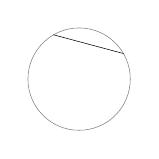
\begin{tikzpicture}[scale=0.65]
\tkzDefPoints{0/0/O}
\tkzDefShiftPoint[O](30:1){A}
\tkzDefShiftPoint[O](120:1){B}
\tkzDrawCircle(O,A)
\tkzDrawSegment(A,B)
\end{tikzpicture}
\end{tcolorbox}
\smallskip 

\begin{tcolorbox}[colframe=black!20!white, opacitybacktitle=0.1, coltitle=black, title=\textbf{Congruent Central Angles and Chords}]
In the same circle or congruent circles, two minor arcs are congruent if and only if their corresponding central angles are congruent. \newline 

\begin{minipage}{0.5\textwidth}
\begin{itemize}
    \item $\angle AOB \cong \angle COD \longleftrightarrow \overline{AB} \cong \overline{CD}$
\end{itemize}
\end{minipage}
\begin{minipage}{0.4\textwidth}
    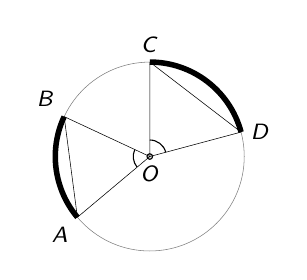
\begin{tikzpicture}[scale=0.6]
    \tkzDefPoints{0/0/O, 0/2/C}
    \tkzDefShiftPoint[O](15:2){D}
    \tkzDefShiftPoint[O](155:2){B}
    \tkzDefShiftPoint[O](220:2){A}
    \tkzDrawCircle(O,A)
    \tkzDrawPoint(O)
    \tkzDrawPolygon(O,C,D)
    \tkzMarkAngle[size=0.35](D,O,C)
    \tkzMarkAngle[size=0.35](B,O,A)
    \draw [line width = 2] (15:2) arc (15:90:2);
    \draw [line width = 2] (155:2) arc (155:220:2);
    \tkzDrawPolygon(O,A,B)
    \tkzLabelPoints[below](O)
    \tkzLabelPoints[below left](A)
    \tkzLabelPoints[right](D)
    \tkzLabelPoints[above](C)
    \tkzLabelPoints[above left](B)
    \end{tikzpicture}
\end{minipage}
\end{tcolorbox}
\smallskip 

\begin{tcolorbox}[colframe=black!20!white, opacitybacktitle=0.1, coltitle=black, title=\textbf{Congruent Chords and Arcs}]
In the same circle or congruent circles, two minor arcs are congruent if and only if their corresponding chords are congruent.\newline 

\begin{minipage}{0.5\textwidth}
\begin{itemize}
    \item $\overline{AB} \cong \overline{CD} \longleftrightarrow \arc{\textit{AB}} \cong \arc{\textit{CD}}$
\end{itemize}
\end{minipage}
\begin{minipage}{0.4\textwidth}
    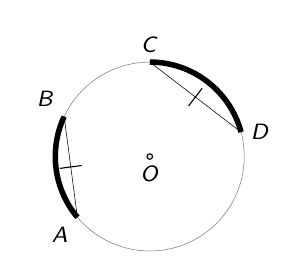
\begin{tikzpicture}[scale=0.6]
    \tkzDefPoints{0/0/O, 0/2/C}
    \tkzDefShiftPoint[O](15:2){D}
    \tkzDefShiftPoint[O](155:2){B}
    \tkzDefShiftPoint[O](220:2){A}
    \tkzDrawCircle(O,A)
    \tkzDrawPoint(O)
    \tkzDrawSegments(A,B C,D)
    \tkzMarkSegments[mark=|](A,B C,D)
    \tkzLabelPoints[below](O)
    \tkzLabelPoints[below left](A)
    \tkzLabelPoints[right](D)
    \tkzLabelPoints[above](C)
    \tkzLabelPoints[above left](B)
    \draw [line width = 2] (15:2) arc (15:90:2);
    \draw [line width = 2] (155:2) arc (155:220:2);
    \end{tikzpicture}
\end{minipage}
\end{tcolorbox}

\begin{example}
In the figures, $\odot J \cong \odot K$ and $\arc{\textit{MN}} \cong \arc{\textit{PQ}}$. Find $PQ.$
\newline\\

\begin{tabular}{p{0.35\textwidth}p{0.35\textwidth}}
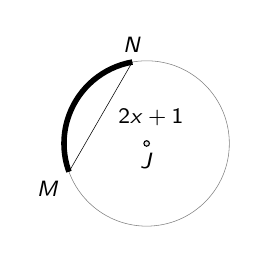
\begin{tikzpicture}[scale=0.6]
\tkzDefPoints{0/0/J}
\tkzDefShiftPoint[J](100:1.75){N}
\tkzDefShiftPoint[J](200:1.75){M}
\tkzDrawPoint(J)
\tkzDrawCircle(J,N)
\tkzDrawSegment(M,N)
\draw [line width = 2] (N) arc (100:200:1.75);
\tkzLabelSegment[right, xshift=0.1cm](M,N){\footnotesize $2x+1$}
\tkzLabelPoints[below](J)
\tkzLabelPoints[above](N)
\tkzLabelPoints[below left](M)
\end{tikzpicture}
&
\begin{tikzpicture}[scale=0.6]
\tkzDefPoints{0/0/K}
\tkzDefShiftPoint[J](30:1.75){Q}
\tkzDefShiftPoint[J](130:1.75){P}
\tkzDrawPoint(K)
\tkzDrawCircle(K,P)
\tkzDrawSegment(P,Q)
\draw [line width = 2] (Q) arc (30:130:1.75);
\tkzLabelSegment[below, yshift=-0.1cm](P,Q){\footnotesize $3x-7$}
\tkzLabelPoints[below](K)
\tkzLabelPoints[left](P)
\tkzLabelPoints[right](Q)
\end{tikzpicture}
\end{tabular}
\end{example}

\begin{tcolorbox}[colframe=black!20!white, opacitybacktitle=0.1, coltitle=black, title=\textbf{Bisecting Arcs and Chords}]
If a diameter (or radius) is perpendicular to a chord, then it bisects the chord and its arc (and vice versa).\newline 

\begin{minipage}{0.5\textwidth}
\begin{itemize}
    \item If $\overline{CD} \perp \overline{AB}$ then
    \begin{itemize}
        \item $\overline{AE} \cong \overline{BE}$
        \item $\arc{AC} \cong \arc{BC}$
    \end{itemize}   
    \smallskip
    \item If $\overline{AE} \cong \overline{BE}$ and $\arc{\textit{AC}} \cong \arc{\textit{BC}}$ then
    \begin{itemize}
        \item $\overline{CD} \perp \overline{AB}$
    \end{itemize}
\end{itemize}
\end{minipage}
\begin{minipage}{0.4\textwidth}
    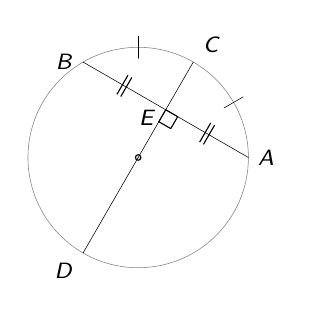
\begin{tikzpicture}[scale=0.7]
    \tkzDefPoints{0/0/O, 2/0/A}
    \tkzDrawCircle(O,A)
    \tkzDefShiftPoint[O](120:2){B}
    \tkzDrawPoint(O)
    \tkzLabelPoints[right](A)
    \tkzLabelPoints[left](B)
    \tkzDefShiftPoint[O](60:2){C}
    \tkzDefShiftPoint[O](240:2){D}
    \tkzDrawSegments(A,B C,D)
    \tkzLabelPoints[above right](C)
    \tkzLabelPoints[below left](D)
    \tkzInterLL(A,B)(C,D) \tkzGetPoint{E}
    \tkzLabelPoints[left, yshift=-0.1cm](E)
    \tkzMarkSegments[mark=||](A,E B,E)
    \tkzMarkRightAngle(A,E,D)
    \tkzDefShiftPoint[O](90:1.8){F}
    \tkzDefShiftPoint[O](90:2.2){G}
    \tkzDrawSegment(F,G)
    \tkzDefShiftPoint[O](30:1.8){H}
    \tkzDefShiftPoint[O](30:2.2){I}
    \tkzDrawSegment(H,I)
    \end{tikzpicture}
\end{minipage}
\end{tcolorbox}
\bigskip 

\begin{example}
In $\odot S$, $m\arc{\textit{PQR}} = 98$. Find $m\arc{\textit{PQ}}$ and $PR$.
\newline

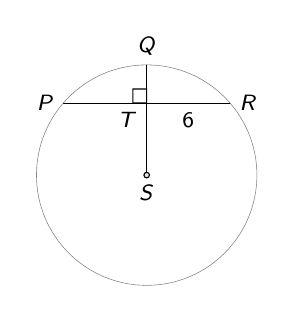
\begin{tikzpicture}[scale=0.7]
\tkzDefPoints{0/0/S, 0/2/Q}
\tkzDrawCircle(S,Q)
\tkzDefShiftPoint[S](41:2){R}
\tkzDefShiftPoint[S](139:2){P}
\tkzDrawSegments(S,Q P,R)
\tkzInterLL(S,Q)(P,R)   \tkzGetPoint{T}
\tkzLabelPoints[below](S)
\tkzLabelPoints[right](R)
\tkzLabelPoints[above](Q)
\tkzLabelPoints[left](P)
\tkzLabelPoints[below left](T)
\tkzDrawPoint(S)
\tkzLabelSegment[below](T,R){6}
\tkzMarkRightAngle(Q,T,P)
\end{tikzpicture}
\end{example}

\begin{example}
Find the length of each.
\begin{multicols}{2}
\begin{enumerate}[(a)]
    \item Find $JL$ if $GH=30$ and $KM=22$.
    \item Find $TV$.
\end{enumerate}
\end{multicols}
\begin{minipage}{0.5\textwidth}
    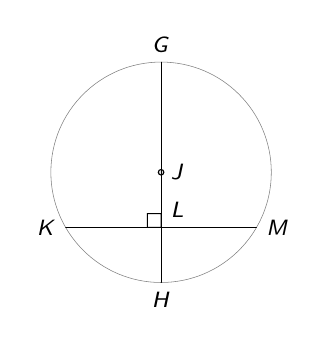
\begin{tikzpicture}[scale=0.7]
    \tkzDefPoints{0/0/J, 0/2/G, 0/-2/H}
    \tkzDrawCircle(J,G)
    \tkzDrawPoint(J)
    \tkzDefShiftPoint[J](210:2){K}
    \tkzDefShiftPoint[J](330:2){M}
    \tkzDrawSegments(G,H K,M)
    \tkzLabelPoints[above](G)
    \tkzLabelPoints[below](H)
    \tkzLabelPoints[left](K)
    \tkzLabelPoints[right](M,J)
    \tkzInterLL(G,H)(K,M)   \tkzGetPoint{L}
    \tkzLabelPoints[above right](L)
    \tkzMarkRightAngle(J,L,K)
    \end{tikzpicture}
\end{minipage}
\begin{minipage}{0.4\textwidth}
    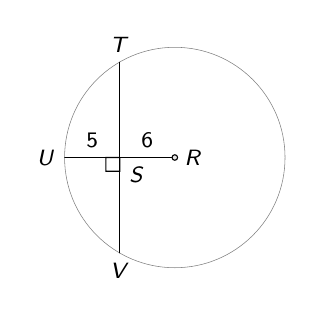
\begin{tikzpicture}[scale=0.7]
    \tkzDefPoints{0/0/R, -2/0/U}
    \tkzDrawCircle(R,U)
    \tkzDefShiftPoint[R](120:2){T}
    \tkzDefShiftPoint[R](240:2){V}
    \tkzDrawSegments(R,U T,V)
    \tkzInterLL(R,U)(T,V)   \tkzGetPoint{S}
    \tkzMarkRightAngle(U,S,V)
    \tkzDrawPoint(R)
    \tkzLabelPoints[right](R)
    \tkzLabelPoints[above](T)
    \tkzLabelPoints[left](U)
    \tkzLabelPoints[below](V)
    \tkzLabelPoints[below right](S)
    \tkzLabelSegment[above](R,S){6}
    \tkzLabelSegment[above](U,S){5}
    \end{tikzpicture}
\end{minipage}
\end{example}

\begin{tcolorbox}[colframe=black!20!white, opacitybacktitle=0.1, coltitle=black, title=\textbf{Equidistant Chords Theorem}]
In the same circle or congruent circles, two chords are congruent if and only if they are equidistant from the center. \newline 

\begin{minipage}{0.5\textwidth}
\begin{itemize}
    \item If $OE = OF$ then $\overline{AB} \cong \overline{CD}$
    \item If $\overline{AB} \cong \overline{CD}$ then $OE = OF$
\end{itemize}
\end{minipage}
\begin{minipage}{0.4\textwidth}
    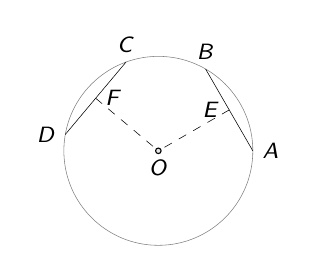
\begin{tikzpicture}[scale=0.6]
    \tkzDefPoints{0/0/O, 2/0/A}
    \tkzDrawCircle(O,A)
    \tkzDrawPoints(O)
    \tkzDefShiftPoint[O](60:2){B}
    \tkzDefShiftPoint[O](110:2){C}
    \tkzDefShiftPoint[O](170:2){D}
    \tkzDrawSegments(A,B C,D)
    \tkzLabelPoints[right](A)
    \tkzLabelPoints[above](B)
    \tkzLabelPoints[above](C)
    \tkzLabelPoints[left](D)
    \tkzLabelPoints[below](O)
    \tkzDefMidPoint(A,B)    \tkzGetPoint{E}
    \tkzDrawSegment[dashed](E,O)
    \tkzDefMidPoint(C,D)    \tkzGetPoint{F}
    \tkzDrawSegment[dashed](F,O)
    \tkzLabelPoints[right](F)
    \tkzLabelPoints[left](E)
    \end{tikzpicture}
\end{minipage}
\end{tcolorbox}
\bigskip 

\begin{example}
\begin{multicols}{2}
    \begin{enumerate}[(a)]
        \item Find $AB$ if $WX=XY=22$.
        \item Find $x$ if $PQ=3x-4$ and $RS=14$.
    \end{enumerate}
\end{multicols}
\begin{minipage}{0.5\textwidth}
    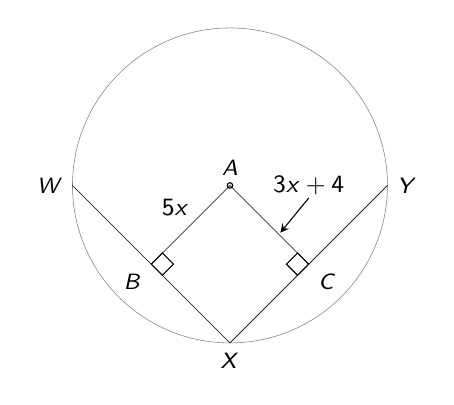
\begin{tikzpicture}[scale=0.8]
    \tkzDefPoints{0/0/A, -2.5/0/W, 2.5/0/Y, 0/-2.5/X}
    \tkzDrawCircle(A,W)
    \tkzDrawPoint(A)
    \tkzDrawSegments(W,X Y,X)
    \tkzDefMidPoint(W,X)    \tkzGetPoint{B}
    \tkzDefMidPoint(Y,X)    \tkzGetPoint{C}
    \tkzDrawSegments(A,B A,C)
    \tkzLabelPoints[above](A)
    \tkzLabelPoints[left](W)
    \tkzLabelPoints[below left](B)
    \tkzLabelPoints[below](X)
    \tkzLabelPoints[below right](C)
    \tkzLabelPoints[right](Y)
    \tkzMarkRightAngles(A,B,X A,C,X)
    \tkzLabelSegment[above left, xshift=0.1cm](A,B){\small $5x$}
    \node at (1.25,0) {\small $3x+4$};
    \draw [->, >=stealth] (1.25,-0.2) -- (0.8,-0.75);
    \end{tikzpicture}
\end{minipage}
\begin{minipage}{0.4\textwidth}
    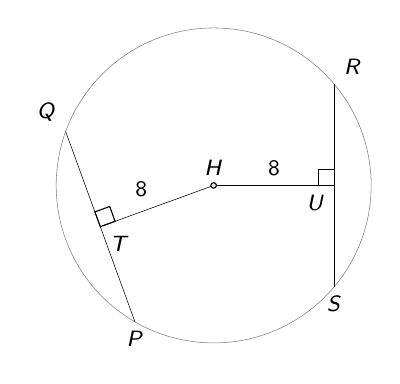
\begin{tikzpicture}[scale=0.8]
    \tkzDefPoints{0/0/H}
    \tkzDefShiftPoint[H](40:2.5){R}
    \tkzDefShiftPoint[H](-40:2.5){S}
    \tkzDefShiftPoint[H](160:2.5){Q}
    \tkzDefShiftPoint[H](240:2.5){P}
    \tkzDrawCircle(H,Q)
    \tkzDefMidPoint(Q,P)    \tkzGetPoint{T}
    \tkzDefMidPoint(R,S)    \tkzGetPoint{U}
    \tkzDrawSegments(Q,P R,S H,T H,U)
    \tkzDrawPoint(H)
    \tkzLabelPoints[above](H)
    \tkzLabelPoints[above left](Q)
    \tkzLabelPoints[above right](R)
    \tkzLabelPoints[below](P,S)
    \tkzLabelPoints[below right](T)
    \tkzLabelPoints[below left](U)
    \tkzMarkRightAngles(H,T,Q H,U,R)
    \tkzLabelSegment[above left](H,T){8}
    \tkzLabelSegment[above](H,U){8}
    \end{tikzpicture}
\end{minipage}
\end{example}
\end{document}
